%!TEX root = ../main.tex
%%%%%%%%%%%%%%%%%%%%%%%%%%%%%%%%%%
% Links:
%
% Difficulty: Companies: 
%%%%%%%%%%%%%%%%%%%%%%%%%%%%%%%%%%


%\begin{figure} \centering
%   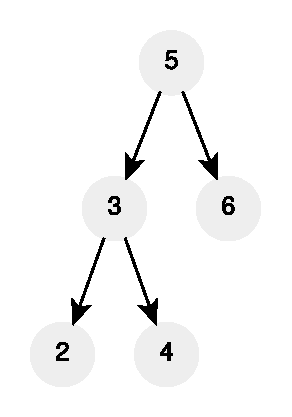
\includegraphics[width=\textwidth]{sources/next_greater_element/images/example1} \caption[Sample
%   short cpation]{Sample Caption}. \label{fig:next_greater_element:example1} \end{figure}

\chapter{Next Greater Element \RN{1}}
\label{ch:next_greater_element}
\section*{Introduction}
One of the key steps in consistent hashing\footnote{A special type of hashing that avoids having to remap every entry in the hash-table when the bucket size changes (to the contrary of what happens when map keys and buckets via a modular operation). The classic example of its usage is in load-balancing or caching in a distributed environment where a distributed hash-map is to be maintained across a number of machines. One way of distributing objects evenly across the $n$ machines is to place data $o$ into the machine $h(o) \Mod (n)$.
However, if a server is added/removed, the server assignment of a lot of the data in all machines may change.
This is problematic since servers often go up or down and each and that would cause a large amount of cache misses. }
is when we have to retrieve the IP of the machine some data $o$ resides in and in a nutshell works by  first calculating the hash of the data itself $h(o)$ and then find the smallest hashkey $h(s)$ for a server that is larger than $h(o)$.
This operations might be performed thousands of times per seconds in a large system and it is therefore quite important to make it as fast as possible. 

In this chapter we will analyze a similar problem where we are given a bag of integers and we need to find the \textit{next greater} element for each of them. The number of applications and variations is high and we feel this problem is a must and that the tecniques shown in this chapter can be applicable to a other real-life coding interview problem bein asked out there in the wild. 

\section{Problem statement}
\begin{exercise}
\label{example:next_greater_element:exercice1}
Write a function that  - given two arrays with no duplicates $A$ and $B$ where $A \subset B$  - returns an
array $C$ of size $|A|$ where $C_i$ contains the next greater element of $A_i$ among the elements of
$B$. The next greater element of a number $A_i$ is defined as the smallest element greater than
$A_i$ among the elements of $B$ from index $j$ to $|B|-1$ where $B_j = A_i$

In other words, for each $A_i$ the function finds the smallest element in $B$ that is greater than
$A_i$ among the cells that are to the right of the cell in $B$ having the value $A_i$ and places it
into $C$ at index $i$.

	%example1
	\begin{example}
		\label{example:next_greater_element:example1}
		\hfill \\
		Given $A=\{4,1,2\}$ and $B=\{1,3,4,2\}$ the function returns $C=\{-1,2,-1\}$. $C_0 = -1$
		because there $A_0 = 4$ appears in $B$ at index $2$ and there is no cell to the right of
		$B_2$ that is strictly greater than $4$. $C_1 = 2$ and because $1$ appears in $B$ at index $0$
		and the smallest element larger than $1$ after index $0$ in $B$ is the element $2$ in the
		last position. $C_2 = -1$ because $A_2 = 2$ appears in $B$ at index $3$ and there is no
		element to the right of it. Note that there exists a value in $B$ that is larger than $2$
		but we are not considering it because it appears to the left of the cell in $B$ holding
		value $A_2=2$.
		
	\end{example}

	%example2
	\begin{example}
		\label{example:next_greater_element:example2}
		\hfill \\
		Given $A=\{2,4\}$ and $B=\{9,2,1,4,12,8\}$ the function returns $C=\{4,8\}$. $C_0 = 4$
		because there $A_0 = 2$ appears in $B$ at index $1$ and the smallest element larger than
		$2$ in $B$ from the cell to the right of the one at index $1$ is $4$.
		
		$C_1 = 8$ because there $A_0 = 4$ appears in $B$ at index $3$ and  the smallest element
		larger than $2$ in $B$ from the cell to the right of the one at index $3$ is $8$, appearing
		at the very end of $B$. Note that $12$ is also larger than $4$ and appears to the right
		of the index $3$ but is not the correct answer because it is not the smallest.
	\end{example}
\end{exercise}

\section{Clarification Questions}

\begin{QandA}
	\item \begin{questionitem} \begin{question} How should the function behave when an element of $A$ does not have a next greater in $B$?  \end{question} 	 
    \begin{answered}
		\textit{The function can insert $-1$ in the corresponding cell of $C$.}
	\end{answered} \end{questionitem}
	
\end{QandA}

\subsection{Brute-force}
\label{next_greater_element:sec:bruteforce}
This problem has a very intuitive brute-force solution that can be broken down into the following steps:
\begin{enumerate}
	\item looping through each element at index $i$ of $A$
	\item finding the position $j$ in $B$ where the value $A_i$ appears i.e. $B_j = A_i$ (which
	exists because $A \subset B$)
	\item finding the smallest element larger than $A_i$ in $B$ only considering those positions strictly
	after $j$.
\end{enumerate}
An implementation of this approach is shown in Listing \ref{list:next_greater_element:bruteforce}
where we use \inline{std::find} to the location in $B$ (the iterator \inline{it}) where $A_j$
exists. The subsequent \inline{while} is used to scan the remainder of the array and to keep track
of the smallest element that is larger than $A_i$. The complexity of this approach is $O(|A| \times
|B|)$ as we could potentially do linear  work (proportional to $|B|$) for each  element of
$A$. One such case is when the elements of $A$ appear in the first positions of $B$. 
\lstinputlisting[language=c++, caption={Brute-force solution to the \textit{next smaller element}.},label=list:next_greater_element:bruteforce]{sources/next_greater_element/next_greater_element_solution1.cpp}


\section{$O(|B|log(|B|))$ time, $O(|B|)$ space solution}
\label{next_greater_element:sec:nlogntime}
We can solve this problem much faster than quadratic time if, as is often the case,  we are willing to use some additional
space. In particular the problem is easily solved if we have
a map containing the information about the next greater element for each of the elements of $B$. We
could then simply loop over all the elements of $A$ and query such a map to get the required answer.
However that does raise the question: how can we generate such a map?

The idea is that we can fill the map for each element of $B$ starting from the back and at the same
time keep a sorted list of all the elements of $B$ that we have already processed. This list can be
used to quickly (by doing a binary search on it) find the upper bound for a given value. The upper
bound for an integer $x$ is the first (or smallest) element in a collection that is strictly larger
than $x$. The upper bound operation can be easily implemented on a sorted collection using binary
search. We have already implemented a similar operation (the lower bound) in Chapter
\ref{ch:find_k_closest_in_array} and you can check Listing
\ref{list:find_k_closest_in_array:binary_lower_bound} (at page
\pageref{list:find_k_closest_in_array:binary_lower_bound}) to have an idea of how you can go about
brewing  your own version of \inline{upper_bound}.


The idea described above is implemented in Listing \ref{list:next_greater_element:set}. The
\inline{std::set<int> N} contains the sorted list of elements of $B$ that we have already processed
while the \inline{std::unordered_map<int,int> C_val} contains the information about the upper bounds
for each of the processed elements of $B$. The first \inline{for} goes through each element $j$ of
$B$ (from the back to the front) and calculates the answer for $B_j$ by looking into the sorted
\inline{std::set} $N$\footnote{Note that we do not use the free function
\href{https://en.cppreference.com/w/cpp/algorithm/upper_bound}{\inline{std::upper_bound}} because on
non linear data structures (like \inline{std::set}) it operates in linear time instead of
logarithmic time.}. The second \inline{for} loop only takes care of copying the relevant information
from the map \inline{C_val} to the return array. The time and space complexity of this code are
$O(|B|log(|B|))$ (each of the $|B|$ insertions in $N$ costs $O(log(|B|)$) and $O(|B|)$,
respectively.

\lstinputlisting[language=c++, caption={$O(nlog(n))$ time and linear space solution.},label=list:next_greater_element:set]{sources/next_greater_element/next_greater_element_solution2.cpp}

\section{Common Variation}
\subsection{First next greater element}
\label{next_greater_element:sec:first}
There is a common variation of this problem featuring an almost identical statement to the one shown
in Section \ref{} with the only difference being that for an element of $A_i$ we should return the
first (and not the necessarily the smallest as in the original variant) element in $B$ that is
greater than $A_i$.

\begin{exercise}
	\label{example:next_greater_element:exercice2}
	Write a function that -  given two arrays with no duplicates $A$ and $B$ where $A \subset B$ - 
	returns an array $C$ of size $|A|$ where $C_i$ contains the first element greater than $A_i$
	among the elements of $B$ strictly after the cell at index $j$, where $B_j = A_i$.
	
	In other words, for each $A_i$ the function finds the first element in $B$ that is greater than
	$A_i$ among the cells that are to the right of the cell in $B$ having the value $A_i$ and places
	it into $C$ at index $i$.

\end{exercise}

\section{Discussion}
\label{next_greater_element:sec:variation1:discussion}
The difference with the original variation is minimal but big enough such that we have a
linear-time solution for this version of the problem. While in solving the original problem  we were forced to keep a
sorted list of all the already processed elements of $B$, this time we can simply keep a stack
storing only those processed elements of $B$ so that they form an increasing sequence.

Suppose we have a decreasing sequence followed by a greater number. For example, consider the
following list: $\{7,8,5, 4, 3, 2, 1, 6\}$ (see Figure \ref{fig:next_greater:stack});
initially the stack is empty and when we process the
first number ($6$) there  is clearly no greater element to its right. As the stack is empty,
adding $6$ to it would still preserve the fact that the numbers contained in it form an increasing
sequence (see Figure \ref{fig:next_greater:variation1:stack1}).
When the $1$ is processed then the stack is not empty and $6$ is at the top which is larger
than $1$. Therefore we can use $6$ as an answer for $1$ and add $1$ to the stack because the
sequence $1,6$ is still increasing (see Figure \ref{fig:next_greater:variation1:stack2}). Things however, are a bit different when $2$ is processed. This
time at the top of the stack we find a $1$ which is smaller than $2$. As such,  the top of the
stack cannot be the answer for the element $2$. Moreover the sequence $2,1,6$ would not be
increasing and therefore the two cannot be placed on top of the stack as-is. What we do here is remove
the elements from the current stack until placing $2$ at the top
would make the elements in the stack an
increasing sequence. 
So we remove $1$ from the stack and the new stack becomes 
$2,6$ (see Figure \ref{fig:next_greater:variation1:stack3}). 
The rest of the execution is described in more detail in Figure \ref{fig:next_greater:stack}.


From this example we can draw a general approach to solving this problem using a stack. 
When we process an element we try to insert it into the stack paying attention to how this element compares to the top of the stack.
If it is larger then we remove the top of the stack and compare it again with the subsequent element. 
We keep repeating and removing elements from the stack until either the element we are 
trying to place is smaller than the top of the stack or there are no more elements left in the stack.
In the former case then the new top of the stack (after all necessary removals)
is going to be the answer associated with the element we are processing.
In the latter case the answer does not exists and the element we are trying to place on the stack
is therefore the largest processed so far.
Listing \ref{list:next_greater_element:stack} shows an implementation of this idea.


\lstinputlisting[language=c++, caption={linear time solution to the Problem \ref{example:next_greater_element:exercice2} solved using a stack.},label=list:next_greater_element:stack]{sources/next_greater_element/next_greater_element_solution3.cpp}


 \begin{figure}
	\vspace*{-0.5in}
	\centering
	\begin{subfigure}[t]{0.49\textwidth}
		\begin{framed}
			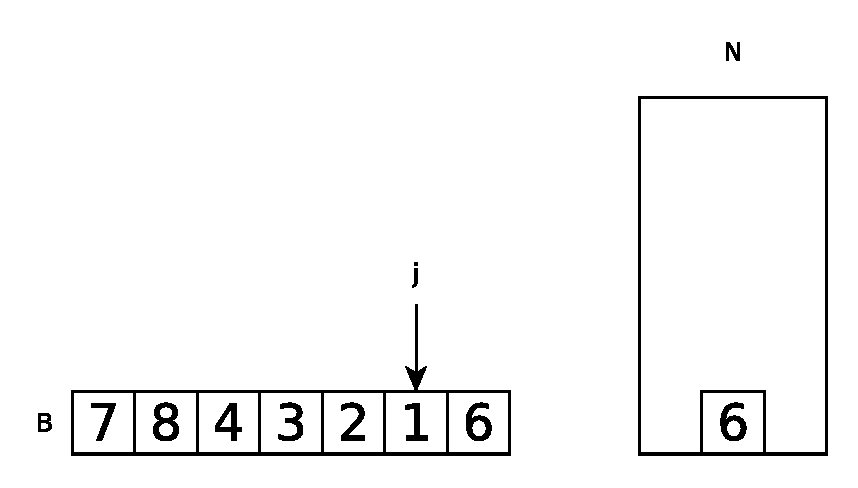
\includegraphics[width=1\linewidth]{sources/next_greater_element/images/stack1}
		\end{framed}
		\caption{The stack is empty. We place $6$ at the top.}
		\label{fig:next_greater:variation1:stack1}
	 \end{subfigure}
	\hfill
	\begin{subfigure}[t]{0.49\textwidth}
		\begin{framed}
			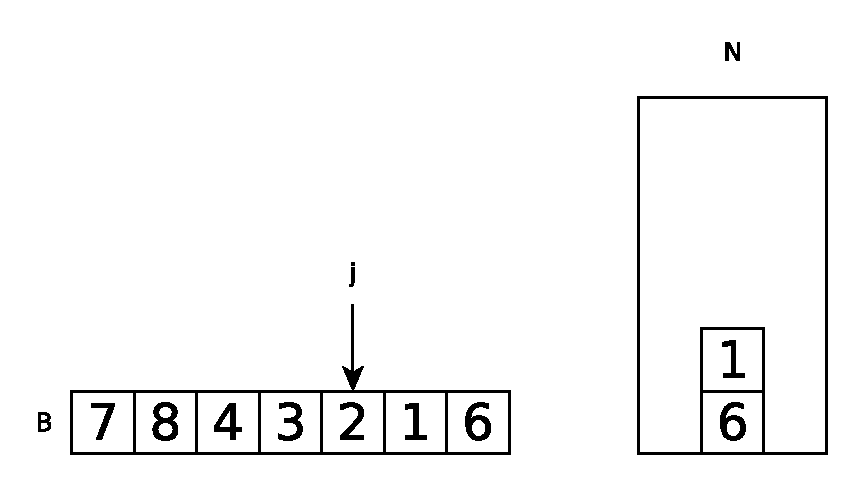
\includegraphics[width=1\linewidth]{sources/next_greater_element/images/stack2}
		\end{framed}
		\caption{$1$ is smaller than the top of the stack therefore $1$ is placed at the top. $6$ is the answer for $1$.}
		\label{fig:next_greater:variation1:stack2}
	 \end{subfigure}
	 \hfill
	 \begin{subfigure}[t]{0.49\textwidth}
		\begin{framed}
			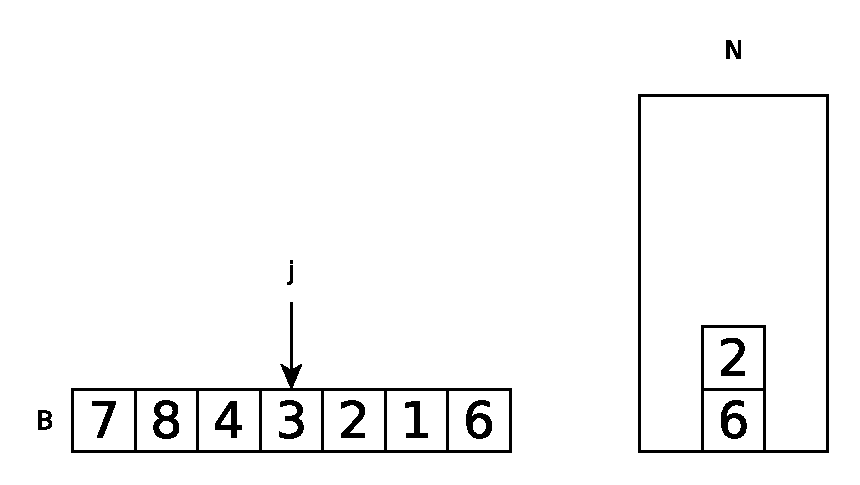
\includegraphics[width=1\linewidth]{sources/next_greater_element/images/stack3}
		\end{framed}
		\caption{The top of the stack $1$ is smaller than $2$. We therefore remove $1$ and place [WHAT]? at the top. $6$, is therefore the answer for $2$}
		\label{fig:next_greater:variation1:stack3}
	 \end{subfigure}
	 \hfill
	 \begin{subfigure}[t]{0.49\textwidth}
		\begin{framed}
			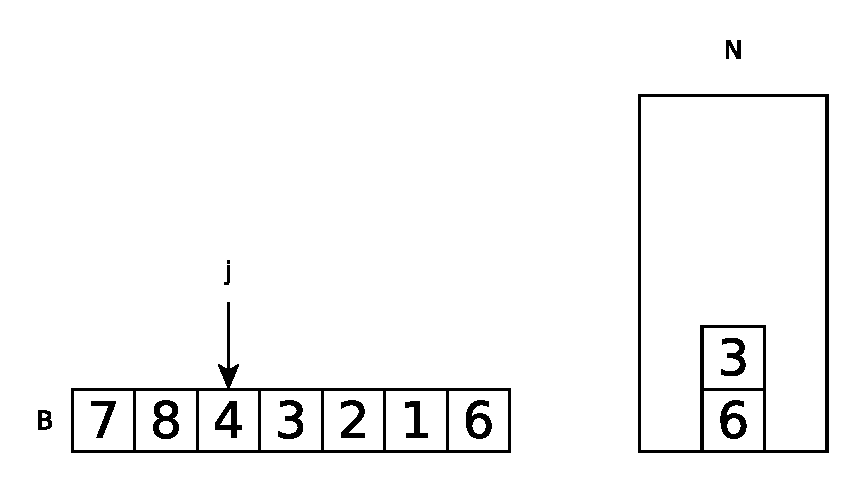
\includegraphics[width=1\linewidth]{sources/next_greater_element/images/stack4}
		\end{framed}
		\caption{Similarly to what we did in Figure \ref{fig:next_greater:variation1:stack3} we remove all the elements at the top until adding the $3$ would preserve the increasing ordering of the stack elements. $2$ is removed and $3$ is the new top. $6$ is the answer for $3$.}
		\label{fig:next_greater:variation1:stack4}
	 \end{subfigure}
	 \hfill
	 \begin{subfigure}[t]{0.49\textwidth}
		\begin{framed}
			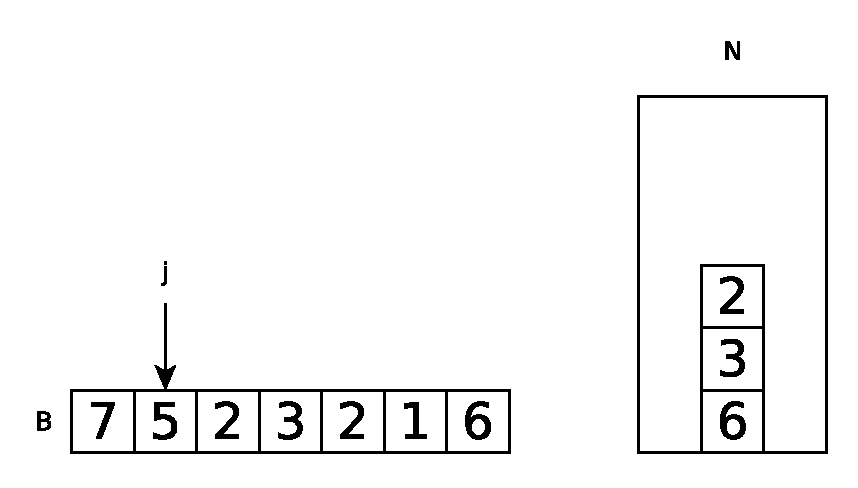
\includegraphics[width=1\linewidth]{sources/next_greater_element/images/stack5}
		\end{framed}
		\caption{We add the $2$ to the stack and return $3$ (the current top of the stack) as the answer for $2$.}
		\label{fig:next_greater:variation1:stack5}
	 \end{subfigure}
	 \hfill
	 \begin{subfigure}[t]{0.49\textwidth}
		\begin{framed}
			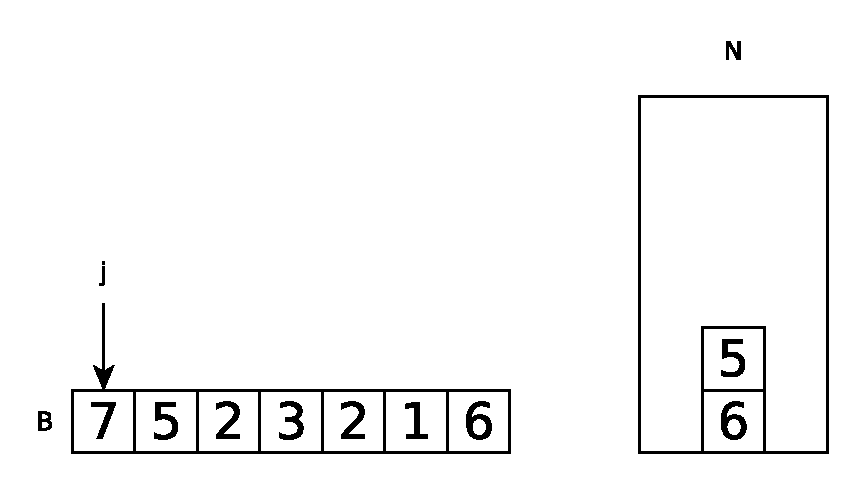
\includegraphics[width=1\linewidth]{sources/next_greater_element/images/stack6}
		\end{framed}
		\caption{$5$ is larger than the first two elements of the stack which are therefore removed.$5$ is the new top and $6$ is the answer for $5$. }
		\label{fig:next_greater:variation1:stack6}
	 \end{subfigure}
	 \hfill
	 \begin{subfigure}[t]{0.49\textwidth}
		\begin{framed}
			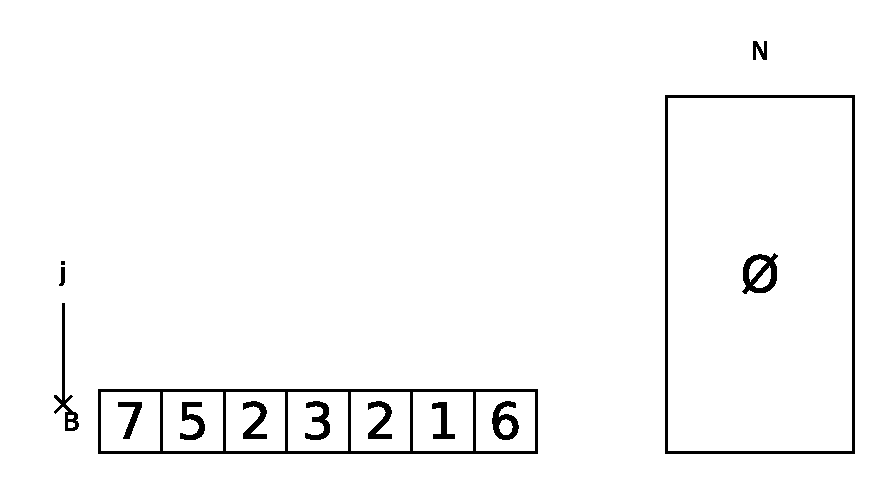
\includegraphics[width=1\linewidth]{sources/next_greater_element/images/stack7}
		\end{framed}
		\caption{$7$ is larger than all the elements currently in the stack. Therefore all the elements are removed and the stack remains empty signalling that $7$ has no greater elements to its right. The process ends here as there are no more elements to process.}
		\label{fig:next_greater:variation1:stack7}
	 \end{subfigure}
	 \caption[]{}
	  \label{fig:next_greater:stack}
\end{figure}